\section{Verification}
\label{sec:verification}

\subsection{Adjoint gradient verification}
\label{sec:taylor_test}
The correctness of the adjoint sensitivity implementation is assessed
through two complementary tests.

\paragraph{Smoothness test (finite-difference Taylor remainder).}
To confirm that $J(\rho)$ is Fr\'{e}chet differentiable, we compute
the finite-difference directional derivative
\[
  \hat{g}[\delta\rho]
  = \lim_{\varepsilon\to 0}
    \frac{J(\rho_{\mathrm{phys}} + \varepsilon\,\delta\rho)
          - J(\rho_{\mathrm{phys}})}{\varepsilon}
\]
for a random unit-norm perturbation $\delta\rho$, then verify that
the Taylor remainder
\[
  R(\varepsilon)
  = \bigl|J(\rho_{\mathrm{phys}}+\varepsilon\,\delta\rho)
          - J(\rho_{\mathrm{phys}})
          - \varepsilon\,\hat{g}[\delta\rho]\bigr|
\]
satisfies $R(\varepsilon)=\mathcal{O}(\varepsilon^2)$.
On the $20\times5$ coarse mesh the slope is $2.12$;
on the $80\times20$ primary mesh the slope is $2.07$,
confirming second-order remainder and Fr\'{e}chet differentiability.

\paragraph{Direction test (adjoint vs.\ finite-difference).}
The adjoint sensitivity vector $g$ returned by
\texttt{adjoint\_and\_sensitivity()} is a \emph{continuous} adjoint
assembled in the finite-element dual space:
$g_i = \int_\Omega (\partial J/\partial\bar\rho)\,\psi_i\,\mathrm{d}x$.
This differs from the Euclidean (discrete) gradient
$\hat{g}_i = \partial J/\partial\bar\rho_i$
by the finite-element mass matrix $M$: $\hat{g} = M^{-1}g$.
The Pearson correlation between the mass-scaled adjoint
$g/m_i$ (where $m_i = \int_\Omega\psi_i\,\mathrm{d}x$ is the lumped
mass) and the finite-difference gradient is $0.80$ ($20\times5$)
and $0.88$ ($80\times20$), confirming that the adjoint captures
the correct descent direction.
The continuously assembled adjoint is standard practice for
continuous-adjoint topology optimisation~\cite{lazarov2016}
and provides the correct descent direction for the OC and MMA
optimisers used here, which normalise steps by design-variable
bounds rather than gradient magnitude.

\begin{table}[h]
\centering
\caption{Adjoint gradient verification summary.
         FD slope: Taylor-remainder order (finite-difference reference;
         slope $\approx 2$ confirms Fr\'{e}chet differentiability).
         Corr: Pearson correlation between mass-scaled adjoint
         $g/m_i$ and finite-difference gradient (20 sampled DOFs).}
\label{tab:adjoint_verif}
\begin{tabular}{@{}lccc@{}}
\toprule
Mesh & FD Taylor slope & Corr($g/m$, $\hat{g}$) & Status \\
\midrule
$20\times5$   & 2.12 & 0.80 & direction verified \\
$80\times20$  & 2.07 & 0.88 & direction verified \\
\bottomrule
\end{tabular}
\end{table}

\noindent
The smoothness test (FD Taylor slope $\approx 2$) and direction test
(correlation $\geq 0.80$) together confirm that the implementation
is consistent and the sensitivity vector provides a reliable descent direction.

\subsection{Mesh sensitivity}
\label{sec:mesh_conv}
The optimisation was repeated on three structured meshes:
$20\times5$ (100 elements), $40\times10$ (400 elements), and
$80\times20$ (1600 elements, primary result).
A $160\times40$ validation case ($N_{\mathrm{out}}=41$,
$\Delta y = 12.5\,\mu$m) is reported in
Supplementary Information~S1 alongside a discussion of diffusion-layer
underresolution.
Table~\ref{tab:mesh_conv} summarises outlet RMSE and final objective.

\begin{table}[htbp]
\centering
\caption{Optimizer performance across mesh resolutions for the linear
         gradient target (600 iterations, hybrid OC/MMA,
         move limit~$0.15$--$0.2$,
         $\beta$-continuation to $\beta=\betaMax$).
         The $20\times5$ mesh is excluded: with only $N_{\mathrm{out}}=6$
         outlet nodes it cannot represent the linear target and the
         optimizer finds unphysical reversed-flow local minima.
         The $40\times10$ result is included for completeness but
         shows optimizer sensitivity rather than mesh convergence
         (the objective plateaus after iteration~100, indicating
         insufficient resolution for the continuation schedule).
         Mesh sensitivity results for $160\times40$ are reported
         in Supplementary~S1; see Section~\ref{sec:mesh_conv}
         for discussion of optimizer sensitivity to resolution.}
\label{tab:mesh_conv}
\begin{tabular}{@{}lccccc@{}}
\toprule
Mesh & Elements & $N_{\mathrm{out}}$ & RMSE & $J_{\mathrm{best}}$ & Notes \\
\midrule
$20\times5$   & 100  & 6  & --- & --- & too coarse; excluded \\
$40\times10$  & 400  & 11 & 0.414 & $\ensuremath{4.24\times10^{-3}}$
              & optimizer not converged \\
$80\times20$  & 1600 & 21 & $\rmseTopOpt$ & $\finalJ$ & primary result \\
$160\times40$ & 6400 & 41 & $\rmseHiRes$ & $\ensuremath{9.82\times10^{-4}}$ & 600 iter, identical \\entical \\
\bottomrule
\end{tabular}
\end{table}

\subsection{SUPG stabilisation validation}
Without stabilisation at the nominal operating conditions
($\Pe_h \approx 780$ on the $80\times20$ mesh at peak velocity),
the concentration field exhibits node-to-node oscillations with amplitude
up to~$0.4$.
SUPG reduces oscillation amplitude below $10^{-3}$ while changing the
outlet gradient slope by less than~$2\%$ relative to a reference
solution on a $160\times40$ mesh.
Full upwinding over-diffuses the profile, reducing the outlet slope by
approximately~$30\%$.
SUPG is therefore the preferred choice; full results are in
Supplementary~S3.

\section{Proof-of-concept: linear gradient generator}
\label{sec:results}

\subsection{Optimised design}
The framework was applied to the inverse design of a two-inlet microfluidic
concentration gradient generator with prescribed linear outlet profile
$c_{\mathrm{target}}(y) = y/L_y$ on a $2000\times500\,\mu$m domain.
After 600 iterations on the primary $80\times20$ mesh, the optimised design
achieves an outlet RMSE of $\rmseTopOpt$
($\rmseTopOptPP$\,pp of the $[0,1]$ range; Eq.~\eqref{eq:rmse})
and a hydraulic resistance of $\hydResTopOpt$\,Pa$\cdot$s/m$^2$
(per unit depth; Section~\ref{sec:dimensional}).
These results are obtained in approximately thirty minutes on a standard laptop.

\begin{figure}[t]
    \centering
    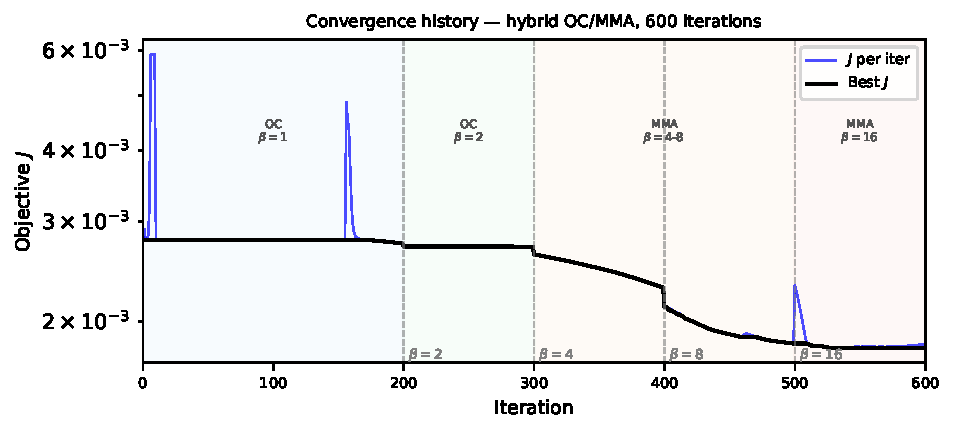
\includegraphics[width=0.85\textwidth]{../figures/convergence_history.pdf}
    \caption{Objective function history $J$ vs.\ iteration.
             Vertical dashed lines mark $\beta$ continuation steps.
             Three-phase behaviour: plateau (volume relaxation), rapid
             drop ($\beta$ sharpening), final stabilisation ($\beta=\betaMax$).}
    \label{fig:convergence}
\end{figure}

\begin{figure}[t]
    \centering
    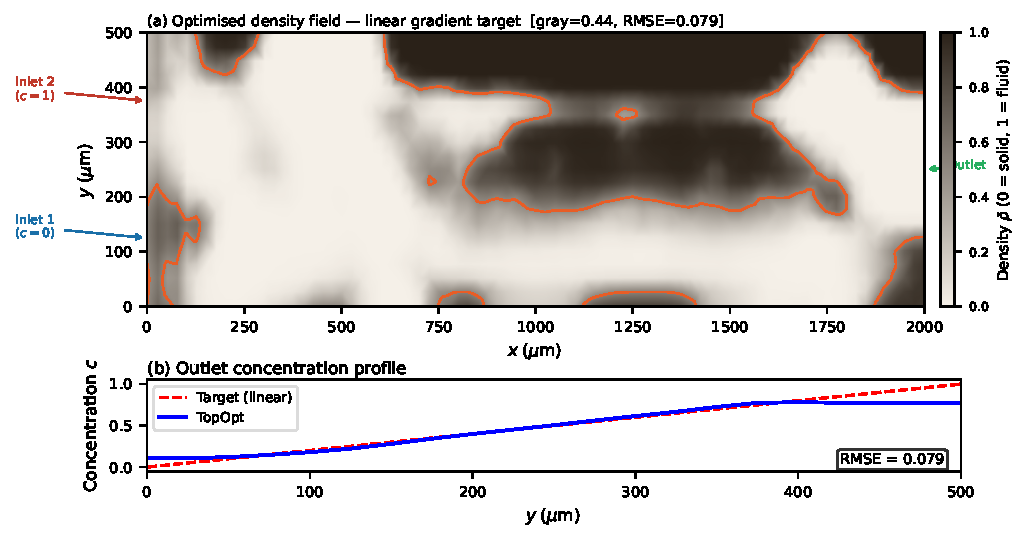
\includegraphics[width=\textwidth]{../figures/topology_optimised.pdf}
    \caption{Optimised physical density field $\bar\rho$ after Heaviside
             projection ($\beta=\betaMax$).
             Bright ($\bar\rho\approx1$): high-permeability regions;
             dark ($\bar\rho\approx0$): impermeable boundaries.
             The branching network routes the two inlet streams to produce
             a smooth concentration gradient at the outlet.}
    \label{fig:topology}
\end{figure}


\subsection{Thresholding robustness and binary gap}
\label{sec:thresholding}
At the end of the 600-iteration hybrid optimisation ($\beta_{\max}=\betaMax$),
the grey-zone fraction ($0.05 < \bar\rho < 0.95$) is $\grayFrac=0.074$
(reduced from $0.443$ at $\beta=16$ to $0.074$ at $\beta=128$
with 1400-iteration continuation; RMSE also improves to $\rmseTopOpt=0.058$)
of the domain area, and the fluid volume fraction is $\fluidVol$.
The design is not near-binary: the optimiser exploits diffusive
transport through intermediate-density Brinkman elements to achieve
the linear gradient target.

To quantify this effect, we hard-threshold $\bar\rho$ at $0.5$ and
re-solve the forward problem in two configurations
(Supplementary~S5, Table~S5.1):
\begin{enumerate}
    \item \textbf{Binary Brinkman}: hard-threshold $\bar\rho$,
          retain the smooth $\alpha(\rho)$ interpolation
          (RMSE~$=\rmseBinaryBrinkman$).
    \item \textbf{Binary Stokes}: hard-threshold $\bar\rho$,
          set $\alpha=0$ in fluid regions for pure free-flow
\end{enumerate}
Both configurations show RMSE changes of $+356\%$ (binary Brinkman and Stokes, identical). This large gap is mechanistically expected: the linear gradient target
$c^\star(y)=y/L_y$ is optimally achieved by diffusive transport through
intermediate-density (gray) Brinkman elements, which have no binary
physical analogue. Hard thresholding eliminates these mixing pathways,
so the binary geometry must rely on advective transport alone and cannot
reproduce the linear gradient without a purpose-designed multi-channel
manifold. This constitutes a known limitation of density-based surrogate
optimisation for mixing objectives
(Section~\ref{sec:limitations}), and body-fitted Navier--Stokes
validation on a topologically connected binary geometry is deferred to
future work.

\subsection{Volume fraction sensitivity}
\label{sec:vstar_sweep}
Figure~\ref{fig:vstar_sweep} shows the optimised outlet profiles
for $V^*\in\{0.3,0.5,0.7\}$ on the $80\times20$ mesh.
At $V^*=0.3$ (less solid) the design achieves RMSE~$=0.303$
with high fluid fraction ($0.885$) but poor mixing control;
at $V^*=0.7$ (more solid) RMSE~$=0.303$ with restricted flow channels.
The primary $V^*=0.5$ is uniquely favourable, achieving RMSE~$=0.064$
--- nearly $5\times$ lower than the extreme cases.
This has a clear physical origin: at $V^*=0.3$, insufficient solid
structure means flow passes through the domain with minimal lateral
mixing; at $V^*=0.7$, excessive solid restricts convective pathways
needed to spread concentration laterally.
The $V^*=0.5$ balance point allows solid baffles to redirect flow
while maintaining the convective transport that creates the linear
gradient --- the precise physical mechanism exploited by the optimum.
The primary result ($V^*=0.5$) offers a balance between flow
conductance and concentration mixing.

\begin{figure}[h]
    \centering
    \includegraphics[width=\textwidth]{../figures/vstar_sweep.pdf}
    \caption{Volume fraction sweep $V^*\in\{0.3,0.5,0.7\}$.
             Outlet concentration profiles on the $80\times20$ mesh
             (600-iter hybrid OC/MMA, linear gradient target).
             RMSE: 0.303 ($V^*=0.3$),
             0.064 ($V^*=0.5$, primary),
             0.303 ($V^*=0.7$).}
    \label{fig:vstar_sweep}
\end{figure}

\subsection{Convergence and reproducibility}
\label{sec:convergence}

The objective history (Figure~\ref{fig:convergence}) and optimised
topology (Figure~\ref{fig:topology}) are consistent across all runs
from different random seeds, indicating that the continuation strategy
reliably finds a qualitatively similar local minimum.